
\noindent\begin{minipage}{\textwidth}
    \begin{table}[H]
        \centering
        \caption{Hiperparâmetros e Resultados do Melhor Modelo - swin\_v11\_AM\_opt\_aug}
        \vspace{0.2cm}
        \resizebox{\textwidth}{!}{%
            \begin{tabular}{ll | lrrr}
                \hline
                \multicolumn{2}{c|}{\textbf{Hiperparâmetros}} & \multicolumn{4}{c}{\textbf{Métricas por Classe}} \\ \hline
                \textbf{Parâmetro} & \textbf{Valor} & \textbf{Classe} & \textbf{Precisão} & \textbf{Recall} & \textbf{F1-Score} \\ \hline
    Agendador (\$T\_0\$) & 15 & 31.2 & 0.2687 & 0.8097 & 0.4035 \\ 
Agendador de LR & CosineAnnealingWarmRestarts & 31.3 & 0.2391 & 0.1089 & 0.1497 \\ 
Architecture & swin\_t & 31.4 & 0.4000 & 0.0095 & 0.0186 \\ 
Batch Size & 32 & 32.3 & 0.4231 & 0.1122 & 0.1774 \\ 
Data Augmentation & False & 32.4 & 0.1389 & 0.0862 & 0.1064 \\ 
Decaimento de Peso (WD) & 0.0469 & 33.3 & 0.2706 & 0.1192 & 0.1655 \\ 
Dropout & 0.0301 & 41.4 & 0.0896 & 0.1364 & 0.1081 \\ 
Função de Perda & CrossEntropyLoss & 41.5 & 0.2400 & 0.1538 & 0.1875 \\ 
Hidden Units & 512 & 42.4 & 0.2154 & 0.2059 & 0.2105 \\ 
Label Smoothing & 0.0335 & 44.4 & 0.0701 & 0.3793 & 0.1183 \\ 
\cline{3-6} 
Otimizador & AdamW & \textbf{Média (Macro)} & 0.2097 & 0.2114 & 0.1859 \\ 
Taxa de Aprendizado (LR) & 9.51e-05 & \textbf{MCC} & \multicolumn{3}{c}{0.1454} \\ 
Unfreeze Layers & 3 &  & & &  \\ 
            \hline
            \end{tabular}%
        }
    \end{table}

    \begin{figure}[H]
        \centering
        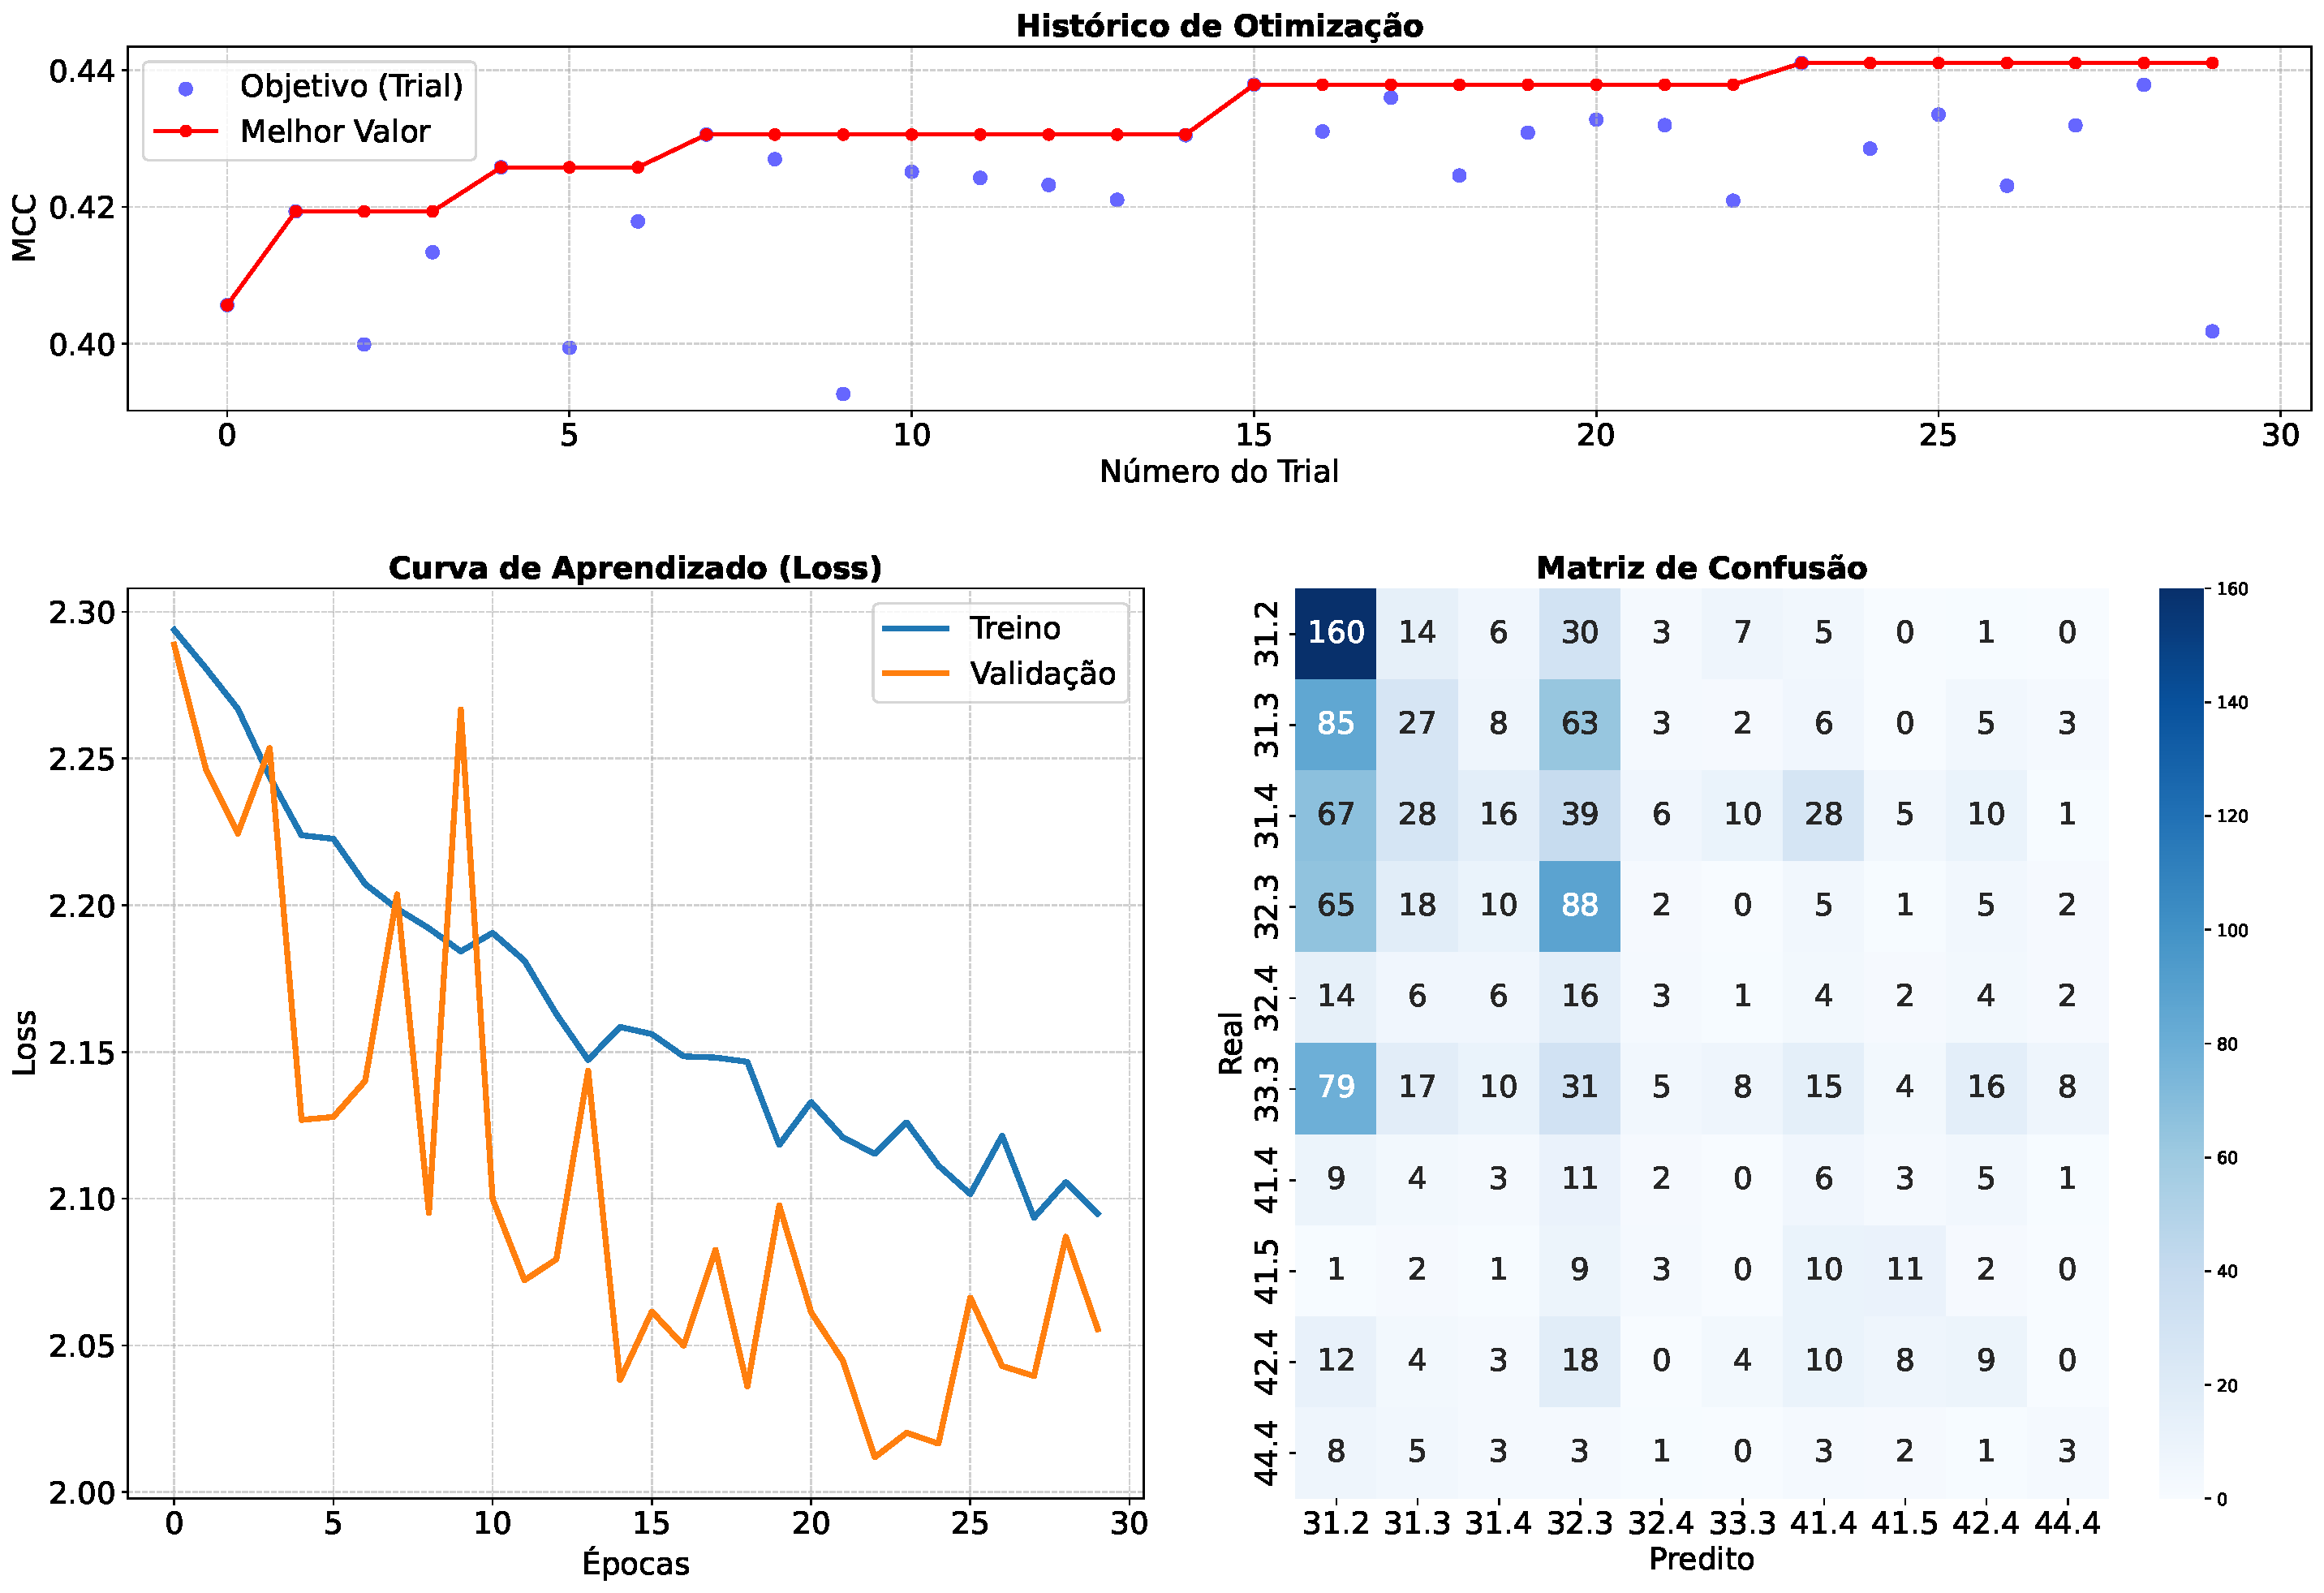
\includegraphics[width=0.85\textwidth]{tex/appendix/experiments/swin_v11_AM_opt_aug/dashboard_consolidado.pdf}
        \caption{Histórico de Otimização, Curvas de Aprendizado e Matriz de Confusão - swin\_v11\_AM\_opt\_aug}
    \end{figure}
\end{minipage}
\clearpage
